\documentclass[12pt]{amsart}
\usepackage{amsmath, amssymb, amsthm, amscd, amsfonts}
\textwidth 6.5 in \oddsidemargin 0 in \evensidemargin 0 in
\textheight 8.5 in \topmargin 0in
\usepackage{pgfplots}
\pgfplotsset{width=10cm,compat=1.9}
\usepackage{url}
\usepackage{tikz}
\usepackage{graphicx}
\usepackage{wrapfig}
\usepackage{multicol}
\usepackage{oz}
\usepackage[
backend=biber,
style=science]{biblatex}
\usepackage{silence}
\usepackage{hyperref}

\newcommand{\VV}{{\mathbb V}}
\newcommand{\RR}{{\mathbb R}}
\newcommand{\CC}{{\mathbb C}}
\newcommand{\ZZ}{{\mathbb Z}}
\newcommand{\QQ}{{\mathbb Q}}
\newcommand{\NN}{{\mathbb N}}
\newcommand{\EE}{{\mathbb E}}
\newcommand{\bfx}{{\bf x}}
\newcommand{\twodots}{\mathinner {\ldotp \ldotp}}

\newtheorem{question}{Question}
\newtheorem{axiom}{Axiom}
\newtheorem{theorem}{Theorem}[section]
\newtheorem{lemma}[theorem]{Lemma}
\newtheorem{corollary}[theorem]{Corollary}
\theoremstyle{definition}
\newtheorem{definition}[theorem]{Definition}
\newtheorem{notation}[theorem]{Notation}
\newtheorem{proposition}[theorem]{Proposition}
\newtheorem{problem}{Problem}
\newtheorem{objective}{Objective}
\newtheorem{example}[theorem]{Example}
\newtheorem{Algorithm}{Algorithm}
\theoremstyle{remark}
\newtheorem{remark}[theorem]{Remark}
\newtheorem{method}[theorem]{Method}
\newtheorem{exercise}{Exercise}

\bibliography{GANpaper}

\begin{document}

\title[Applications of Generative Adversarial Networks]{Applications of Generative Adversarial Networks to Natural Handwriting and Music Creation}

\thanks{The authors, along with their advisor Dana Clahane, are partially supported by NSF-DMS-1541911: RE-C\^{}2\: Research Experiences in Community Colleges.}

\author[K.Little]{Kyle Little}
\email{kylelittle2134@gmail.com}

\author[C.Stevens]{Christopher Stevens}
\email{cestevens@berkeley.edu}

\address{ Mathematics and Computer Science Division, \newline
        Fullerton College, 321 E. Chapman, Fullerton, CA 92832-2095
}

\begin{abstract}
We apply the recent concept of a generative adversarial network (GAN) to two tasks: natural handwriting emulation and music creation.  Because it of great interest to mathematically generalize neural networks (NN's), along the way, we also present some abstract definitions that can serve as templates for NN's and GAN's.
\end{abstract} 

\maketitle
\section{Introduction}

In this paper, we exhibit two applications of so-called generative adversarial networks \cite{1406.2661}, and we attempt to generalize various aspects of them, including even the definition of a neural network.  Before describing GAN's, we will introduce some preliminary notation and definitions in the next sections.  In the sections that follow the section below, we proceed to applications of GAN's to natural handwriting emulation and music creation.  Because the generalization of neural networks is of great interest, along the way, we will take the opportunity to propose general mathematical notions.  The reader will be provided with instructions for playing with our GAN's, along with links to locations where data is stored for experimentation.  We'll also give some examples of outputs of our GAN's in both applications.  For natural handwriting, images are provided, and for natural music creation, we provide links where MIDI files are stored, so that the reader can perhaps be impressed.


\section{Definitions and Notation} 

\begin{notation}[Prediction ($\sim$)]
        Suppose that $p:\RR^{m} \to \RR$ and that $\alpha\in[0,1]$.  Then the
        notation ${\bf v} \sim_\alpha p({\bf v})$, or simply, ${\bf v}\sim p({\bf v})$ in the case that $\alpha=1/2$, 
        denotes the phrase ``The value $p({\bf v})$ allows us to conclude that ${\bf v}\in S$, with 
        probability of truth of this statement being $\geq \alpha$.''  Another way we say this statement can be ``$p({\bf v})$ predicts ${\bf v}$ with probability $\geq 1/2$."  The components of ${\bf v}$ are called {\em predictors.} 
\end{notation}

\begin{example}
        Suppose that $S=[0,\infty)$.  Suppose that $p:\RR\rightarrow[0,1]$ is given by
        \begin{equation*}
        p(x)=\frac{1}{\sqrt{2\pi}}\integral_{-\infty}^x e^{-t^2}dt.
        \end{equation*}
        Then $7.5\sim_{1/2}p(7.5)$ and $7.5\sim p(7.5)$ both denote the same statement, ``The value $p(7.5)$ allows us to conclude that $7.5\in [0,\infty)$, with probability of truth of this statement being $\geq 1/2$.  In this case $7.5$ is a predictor.  The reader who is familiar with the standard normal distribution will recognize here that $p$ here is that distribution, which is the cumulative distribution function of the standard normal (bell) curve.  An elementary statistical computation will show that $p(7.5)=1$.  Thus the statement that $7.5\sim p(7.5)$ can be rewritten as $7.5\sim 1$, which in turn means the same thing as the statement that the value $1$ of the standard normal distribution evaluated at 7.5 indicates that $7.5\in[0,\infty)$, with probability $1$.
\end{example}



To improve our predictions in the specific applications of GANS discussed in this
paper, we must first discuss how to quantify inaccuracy in predictions. To do so,
we attempt to define an error function in the context of the above definition of
prediction.  Later in this paper, we will specialize this idea to the more specific 
applications of Generative Adversarial Networks we are interested in, to natural
handwriting and music creation.

\begin{definition}[Error Function] 
Let 
${\bf x }$ denote an $\RR^n$-valued (datum) variable that we would like to classify as being or not being in a given set $S$, We say that a given function is an {\em error function induced by the variable ${\bf x}$ and ${\bf p}$} and denote such 
an error function by $\EE_{{\bf x}\sim{\bf p}({\bf x})}$ iff the following 
conditions are satisfied in a given classification problem that we are 
interested in:
        \begin{enumerate}
                \item   \begin{align*}
                            \EE_{{\bf x}\sim {\bf p}({\bf x})} : \RR \to \RR,
                        \end{align*}
                \item A given input $d\in\RR$ for this function is the output of $f\circ P$, where $f$ is a one-to-one function on $[0,1]$, and $P$ is a probability function.
                \item $\EE_{{\bf x}\sim{\bf p}({\bf x})}(d)=0$ when the input $d$ corresponds to the statement ${\bf x}\sim_1 p({\bf x})$;
                \item  A large value of $\EE_{{\bf x}\sim{\bf p}({\bf x})}(d)$ for some input $d$ corresponds to the statement that ${\bf x}\sim_\alpha p({\bf x})$ only for small values of $\alpha\geq 0$.
        \end{enumerate}
\end{definition}



In order to make predictions, we must use some mathematical model. For the purpose of GANS, the model we will use is based on the human 
brain's layered neuron activity.  We propose the following way of mathematically defining a neural network:

\begin{definition}[(Generalized) Neural Network]
\begin{enumerate}
\item We call $(V,E,W)$ an {\em neural network}, or, more briefly, an NN, iff the following statements hold:
\begin{enumerate}
\item $(V,E)$ is a digraph.
\item $W$ is a function whose domain is $E$.
\item $\forall (u,v)\in E$ such that $u$ is not the terminal vertex of an edge in $E$, we have that $u$ is a real number.
\item $\forall (u,v)\in E$, $W(u,v):\ $Range$(u)\rightarrow$ Dom$(v)$.
\end{enumerate}
\item An NN $(V,E,W)$ is called {\em real-valued} if and only if every $v\in V$ that is a terminal vertex of some $e\in E$ and  not the initial vertex of some $f\in E$, is a real number.
\item Furthermore, the vertices of an NN that are both the terminal edge of a some vertex in $V$ and the initial edge of another vertex in $V$ are also called {\em neurons}.
\end{enumerate}
\end{definition}

Recall that graphs can be connected or disconnected, or, they can be simple or non-simple.  Since an NN $(V,E,W)$ has an underlying graph $(V,E)$, then NN's can be called, connected, disconnected, simple, or non-simple, in exactly the same manner, depending on the nature of the underlying graph.

However, practically speaking, we note that in reasonable applications, the underlying graph of an NN should be connected and simple.  Since an NN is a mathematical model inspired by the way a brain works, a disconnected NN would be like two separate brains that don't interact with each other (not of interest in this paper).  Furthermore, a non-simple NN would be like a brain with at least one infinite loop of a chain of neurons, which does not happen in nature, and, for algorithms, is something that is obviously undesirable. (We don't want infinite loops in our algorithms.)

For the applications that we are interested in, the vertices of a given neural network that are functions will have domains and ranges in Euclidean space.

\begin{definition}[Euclidean NN and notation within it]
        \begin{enumerate}
        \item We call an NN $(V,E,W)$ {\em Euclidean} iff each $v\in V$ is either a real constant or $v:\RR^m\rightarrow\RR^n$ for some positive integers $m,n$ and, $\forall (u,v)\in E$, we have that $W(u,v)$ is either a real number or a column vector of real numbers whose number of components is the same as the dimension of the domain of $v$.  
        \item Let $(V,E,W)$ be an Euclidean NN, and let $v\in\mathbb{N}$ be the cardinality of $V$.  Denote the vertices by $v_1,v_2,\ldots, v_k$.  
        \begin{enumerate}
                \item We denote by $I:=\{0\twodots k\}$, the set of all integers between and including $0$ and $k$. 
                \item With respect to $m_0,m_1, m_2, \dots, m_k, n_0, n_1, n_2, \dots, n_k \in \mathbb{W}$, the set of all positive integers, we impose that 
                $m_i$ $\forall i$ is the dimension of the domain of $v_i$ vertex and also impose that $n_i$ is the dimension of the range of $v_i$.
                \item That is, we suppose that each vertex $v_i$ of $V$ here satisfies
                \begin{align*}
                                v_i:\mathbb{R}^{m_i} \to \mathbb{R}^{n_i} 
                        \end{align*}
                \item If $i,j\in \{1..k\}$ and $(v_i,v_j)\in E$, then we denote $W(v_i,v_j)$ more briefly by $w_{i,j}$.
        \end{enumerate}
        \end{enumerate}
\end{definition}

The weights we assign each neuron change the network's influence on these neurons. Sometimes, we do not want a neuron to be included in the calculation for training in order to remove dependency on one
neuron. Analogously to the human brain we have certain neurons removed from the graph.

\begin{remark}[Drop-out]
        A weight of zero represents a vertex or neuron has {\em dropped-out} for some training cycle.
        Since the weight is a scalar multiplied by the input vector, when that weight is
        zero, that input will be ignored.
\end{remark}

We have chosen to define neural networks as above to impose a general mathematical structure to the theory of a largely 
implementation-based algorithm. Allowing each neuron to be any function and generalizing weights allows for a general
theoretical neural network definition. A GAN uses two neural networks which are consequently trained in tandem. We will
define the two separate neural networks before we define the full GAN.

\begin{definition}[Perceptron]
        A {\em perceptron} is a neural network consisting of a single layer of weights and
        with identity functions as the vertex set.
\end{definition}

\begin{remark}
        As an effect of this definition, perceptrons may be modeled as linear predictors,
        or as functions ${\bf q}(\bfx)\sim {\bf p}(\bfx)$. Later in the paper we
        will use this notation to refer to perceptrons.
\end{remark}

\begin{definition}[Discriminator]
        A {\em discriminator} is a type of neural network that determines authenticity of input data. It can be
        modeled by a function 
        $$ D:\RR^n \to \RR, $$ together with the other properties of a more general NN.
\end{definition}

The discriminator is some neural network that takes in some vector to check if 
it is a part of the same set as the data it was trained on, and outputs a probability that the
vector is a part of its training set.


\begin{definition}[Generator]
        A {\em generator} is a type of neural network that produces
        new data based on training, and can be described as a function
        $$ G:{\bf z} \to \RR^n $$
        where ${\bf z}$ is a noise vector.
\end{definition}

The generator is some neural network that takes in some kind
of random noise and outputs things that look like the training
data. Thus, when we train our generator in tandem with our
discriminator we can evoke the idea of counterfeiting, in the
sense that the outputs of the generator try to fool
the input to the discriminator.

\section{Definition of a Generative Adversarial Network}

\begin{definition}[Generative Adversarial Network]
        We define a {\em generative adversarial network} (GAN) in terms of a
        two player min-max game between a discriminator $D$ and a
        generator $G$ with value function
        \begin{align*}
                \min\limits_{G}\max\limits_{D}V(D,G) = \mathbb{E}_{{\bf x} \sim p_{data}({\bf x})}[\log D({\bf x})] + 
                \mathbb{E}_{{\bf z} \sim p_{{\bf z}}({\bf z}) } \left[ \log(1-D(G({\bf z}))) \right]\text{  \cite{1406.2661}}
        \end{align*}
        where we train $D$ to maximize the probability of correctly assigning
        labels to both training data and data that comes from $G$. In turn we train $G$
        to minimize $\log(1-D(G({\bf z})))$.
\end{definition}

\section{Results}
\subsection{Natural Handwriting}
The first application of GANs we attempted was to produce handwritten letters and
numbers in a manner that looks human written. We achieved partial results,
based upon and modified from open source work by Diego Gomez\footnote{https://github.com/diegoalejogm/gans}.
Many changes were made in order to preserve outputs long term, as well
as laying foundations for cohesive data inputs. For example, work was first
done using MNIST as the input data, which produced very legible numbers. \\
\begin{center}
    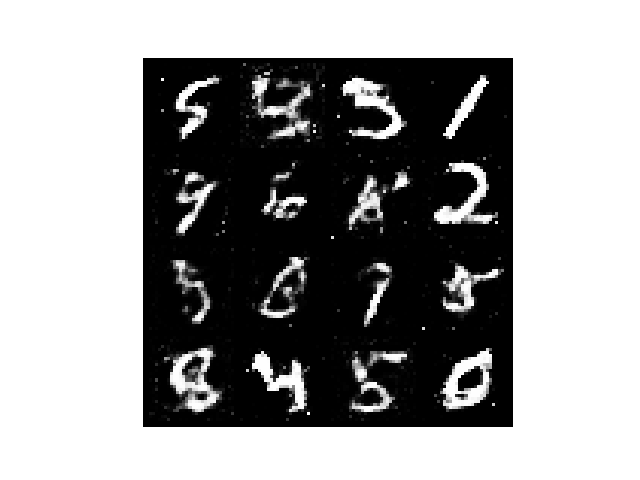
\includegraphics[scale=0.5]{output1.png} \\
\end{center}
The code for the handwriting portion and instructions on how to run it can be found at
\href{https://github.com/Onionchi/GANdwriting}{https://github.com/Onionchi/GANdwriting}

\subsection{Music Creation}
With the second application of GANs we attempted to produce new music based upon 
MIDI files from various classical composers. This involved two neural network models
over the course of our research. Both of these models were useful in finding more about GANs.
Outputs to both models were generally not similar to music that would generally be considered "normal,"
but there was significant improvement between the two models. The model is based off starting code.
\footnote{https://skymind.ai/wiki/generative-adversarial-network-gan}
\\\\
The first model was a naive implementation of a Generative Adversarial network. This model simply took the
input MIDI files and tried to produce new MIDI files that were similar. This led to results that generally fit in one
of two categories.
\\\\
(1). The MIDI file output would be a jumble of notes equivalent to someone randomly pushing 
keys on a keyboard. 
\\\\
(2). The MIDI file output would degrade into two notes one very high pitched and the other very low
pitched. These notes would repeat at seemingly random intervals throughout.
\\\\
We think that these two outcomes are due to a phenomenon known as modal collapse. More specifically over the process
of training GANs, GANs will sometimes after extensive training learn only one way of making output as indicated above.
\\\\
The second model has many improvements over the first. The predictor that used to be a raw note value
was changed to be a difference between notes over time. This way the neural network could try to learn
some form of structure over time in music. This change was very successful and brought about new MIDI
output that had segments resembling musical scales and arpeggios that might be features of human composed music.
\\\\
The code that was written is available publicly at 
\href{https://github.com/Aniranth/GAN_Project}{https://github.com/Aniranth/GAN\_Project}
Simply get Python 3 on your system and follow the instructions in the read-me file of the GitHub.  You can also find sample MIDI files generated by several epochs of testing of the GAN at this link.

\section{Further Research}
There are many different directions that can be taken for further research.
Currently for the application of handwriting we are trying to emulate the handwriting
of Thomas Jefferson, as he has a large volume of annotated written work, available at
the Library of Congress.

We would like to look further into the modal collapse that was experienced in the Music application. 
The authors would specifically like to consider a paper found late found as the  research in this paper developed.\cite{1809.09087}

Another project the authors have significant personal interest in will be to
implement the more generalized neural network that outputs functions rather than
real numbers.

\section{Acknowledgements}
Kyle Little would like to thank Ryan Wilcox for his suggestion to use a change in notes for the note predictor in the second version of the Music application for GANs.

Christopher Stevens would like to thank David Nuon for his helpful conversations
about different types of neural networks.  These conversations helped inspire thought about 
neural networks in the non-traditional view expressed in this paper.


The authors would like to thank Professors Helena Noronha, Bruce Shapiro, and Adriano Zambom of CSUN for their
work organizing this research project and their lectures on data science. As well, we would like
to thank Kevin Scully for several wonderful talks about neural networks at the Fullerton College Mathematics
Colloquium, which inspired our selection of this data science topic for the current project.  The authors would also like to thank the Department of Mathematics at California State University Northridge for providing hospitality and for hosting the Math Research Experiences in Community Colleges Conference for the past three years.  It is exciting to see math research beginning to sprout in community colleges, and data science, the emphasis of this NSF project for the year, is well-chosen for many reasons.

This project was completed as part of Research Experiences in Community Colleges (REC$^2$), which has been funded by the National Science Foundation, under Division of Mathematical Sciences Grant Number 1541911.

\newpage

\printbibliography

\end{document}
